\subsection{Time Measurement on A Single Query Execution}\label{sec:measure_time}

\begin{figure}[th]\centering
\includegraphics[width=0.50\textwidth]{figures/time_measurement.eps}
\caption{Processes considered when timing a query\label{fig:timing}}
\end{figure}

In this section we describe how the time on a single query execution 
is measured. 
There could be in practice quite a few non-DBMS processes simultaneously 
at the time of executing a query. 
Hence, a careful measurement is necessary so that we can later derive 
the time only spent on a DBMS process(es) involving in the single 
query execution (as described in the next subsection). 

First, $GetProcs$() is called to capture all running processes, 
as illustrated in Figure~\ref{fig:timing}. 
To obtain each of the process information, 
the method either iterates {\tt /proc/\{pid\}/stat} or 
takes advantage of {\tt PsList}~\cite{russinovich10}, depending on Unix/Linux 
or Windows operating systems, respectively. 
Once all the information associated with a process 
is extracted, a record of \{process id (pid), command (process name), 
minimum and major faults, cpu time and system time\} is built and mapped 
to the pid to identify the process. 
Subsequently, $GetProcStat$() is invoked to obtain all detailed CPU ticks and 
the max pid at the time of the call. 
The method accesses {\tt /proc/stat} that maintains kernel and system statistics 
(not available on Windows), and it extracts the current 
CPU ticks by user mode, system mode, idle task, wait mode for I/O completion, 
servicing interrupt mode, etc., and lastly the max pid.
The tick information is needed to compute the correct single execution time, 
and the max pid is used to detect the presence of a 
{\em phatom} process(es) in the single query execution (as will be discussed shortly). 
Next, an individual call is made to $GetTime$() right before and 
after executing the query $Q$, thereby measuring the elapsed 
(probably not accurate) time by difference between the start and end times. 
$GetProcStat$() and $GetProcs$() are in turn invoked again after the execution. 
In particular, it is important not to reverse the order of calling 
$GetProcs$() and $GetProcStat$(), in that a phantom process(es), otherwise, 
would be more likely to happen while $GetProcs$() extracts all process information. 
The prevalence of a phantom process(es) included in a single query execution 
could spoil our analysis. 
We will discuss the phantom process in greater detail shortly. 

Now let us consider how the captured processes may influence 
the single query execution. 
As illustrated in Figure~\ref{fig:timing}, 
$P$1, $P$2 and $P$3 are recorded into a map, $M_{1}$ when the first $GetProcs$() 
gets called. 
$P$4 might also appear in $M_{1}$ if $GetProcs$() captures it. 
Another map, $M_{2}$, built by the second $GetProcs$(), 
records $P$3, $P$6 and $P$7, and it might also have $P$8 
for the same reason as $P$4. 
$P$5 is called a phantom process, since it appears and completes 
its task before the query execution is finished. 
$P$5, thus, cannot be captured by $GetProcs$(), but at least we can tell 
whether it would have been present in the query execution 
by comparing the max pids each other extracted by $GetProcStat$(). 
If no difference is made, the query execution data is said to be {\em clean} 
without any phantom process. 
Otherwise, the phantom must have happened during the query execution, so 
the data gets dirty, and thus, it is not considered in our analysis. 

There could be other situations where the execution data cannot be 
used. 
The comparison result with $M_{1}$ and $M_{2}$ reveals that 
$P$1 and $P$2 are not found in $M_{2}$. 
These processes are called {\em stopped} ones. 
It is evident that $P$2 involves the query execution, but it is not easy 
to determine that $P$1 is the same case as $P$2, only by the comparison. 
Therefore, our analysis do not make use of the execution data 
if any stopped processes are detected. 
If $P$4 is captured, it would be counted as a stopped process, and thus, 
the data gets thrown too. 
However, the data would not be unclean although $P$4 is not captured, 
for it does not get involved in the query execution. 

$P$6 and $P$7 are located in $M_{2}$ but not in $M_{1}$. 
Thus, they are said to be {\em started} processes, which could involve 
the query execution. 
Because it is not impossible to get their start times, 
we do not throw the data having started processes. 
Instead, their times will be subtracted from the measured, elapsed time.
To minimize the subtraction as well, 
``{\em infrequently-running} processes'' followed by 
``{\em frequently-running} processes'' are checked in order 
at the first call of $GetProcs$(), and they are checked 
in the other way around at the second call of $GetProcs$() 
when the maps $M_{1}$ and $M_{2}$ are built individually. 

The frequently-running processes mean ones found to be run during 
the execution by the comparison of $M_{1}$ and $M_{2}$. 
For instance, $P$3 could be in the frequently-running process list should it 
show different CPU ticks, thereby proving that it would run during the execution. 
The experiment starts by loading the existing frequently-running process list 
with a small (tunable) number of processes (e.g., 10). 
As the experiment goes, a process could be automatically added to the list 
as long as it did not run last execution but did run this time. 
By adjusting the order of examining processes in $GetProcs$(), 
the tick increase of the running processes could be minimized, and accordingly, 
more accurate query execution time could be computed, minimally 
incurring the subtraction caused by the increase ticks. 
Finally, $P$8 could be classified as a started process once detected. 
It would otherwise be fine since it does not be involved in the query 
execution, either. 

Figure~\ref{alg:exeSpecExp} represents an algorithm of measuring 
the single query execution time as described above. 
Input arguments, $\iterNum$, $\query$, $\prevPlan$ and $\card$, 
denote the current iteration number for repeatability check, 
a given query, the previously detected query plan 
and the current cardinality at which the query gets executed, 
respectively. 
First, the algorithm checks if the given plan, $\prevPlan$ 
is identical to a current plan obtained 
at the time of executing the $\query$ via $GetQueryPlan$(). 
If both plans are inconsistent, then an error is reported. 
Next, to remove cache effects, all the caches from disk through 
operating system to DBMS are flushed.
Before executing $\query$, through $GetProcs$(), $GetProcStat$() and 
$GetTime$() we get $\procMap_{1}$, which 
records all existing process information, 
$cpuStat_{1}$, which stores current CPU ticks and max process ID, and 
$time_{1}$, which gets the current time in milliseconds, in order. 
After finishing the query execution, we again obtain 
$time_{2}$, $cpuStat_{2}$ and $\procMap_{2}$ by calling the above 
methods in reverse order. 
We then get $\mTime$, the measured time on this single query execution, 
and through $\diff$() we receive 
the $\procDiff$ string, which contains executed, started and stopped 
processes during the query execution and their detailed information (increased 
cpu and system times and min and major faults) and the increased CPU ticks 
per entry (such as user and system modes, etc.), if any. 
Lastly, $RecordQueryExecution$() stores all the results, 
$\mTime$ and $\procDiff$ with $\iterNum$, $\query$ and $\card$. 

\begin{figure}[t]
\begin{center}
\begin{algorithmic}
{\bf Algorithm} timeSingleQueryExecution($\iterNum$, $\query$, \\
						\hspace{44.0mm}$\prevPlan$, $\card$):
\STATE $\plan$ $\leftarrow$ $GetQueryPlan$($\query$)
\IF{$\plan$ $\neq$ $\prevPlan$}
	\STATE Error: two different plans are observed \\ 
	at the same cardinality. \\
\ENDIF
\STATE Flush disk drive, OS and DBMS caches. \\
\STATE $\procMap_{1}$ $\leftarrow$ $GetProcs$() \\
\STATE $cpuStat_{1}$ $\leftarrow$ $GetProcStat$() \\
\STATE $time_{1}$ $\leftarrow$ $GetTime$() \\
\STATE $executeQuery$($q$) \\ 
\STATE $time_{2}$ $\leftarrow$ $GetTime$() \\	
\STATE $cpuStat_{2}$ $\leftarrow$ $GetProcStat$() \\
\STATE $\procMap_{2}$ $\leftarrow$ $GetProcs$() \\
\STATE $\mTime$ $\leftarrow$ $time_{2}$ - $time_{1}$ \\	
\STATE $\procDiff$ $\leftarrow$ $\diff$($cpuStat_{1}$, $cpuStat_{2}$, \\
\hspace{22.0mm}							$\procMap_{1}$, $\procMap_{2}$) \\	
\STATE $RecordQueryExecution$($\iterNum$, $\query$, $\card$, \\ 
			\hspace{35.0mm}$\mTime$, $\procDiff$) \\
\end{algorithmic}
\caption{Algorithm for The Single Query Execution Time Measurement\label{alg:exeSpecExp}}
\end{center}
\end{figure}

\subsubsection{Query Execution Time Computation}\label{sec:qe_time}

Figure~\ref{fig:dbms_time} shows the interleaved processes, 
$P_{\other}$ and $P_{\dbms}$, running on a single core. 
$P_{\dbms}$ represents a DBMS-related process, and $P_{\other}$ 
denotes a non-DBMS process. 
To derive the query execution time ($T$) only taken by $P_{\dbms}$, 
the following equation is used: 

\begin{center}
$T$ (ms) = (($U_{\dbms}$+$S_{\dbms}$+$\IO_{\total}$+$\Irq_{\total}$+
$\SoftIrq_{\total}$) - ($\sum_{i=1}^{n}{S_{i}}$)) (ticks) $\times$ 10, 
\end{center}
where $U_{\dbms}$ and $S_{\dbms}$ denote ticks on user and system 
modes of $P_{\dbms}$, and $\IO_{\total}$ and $\Irq_{\total}$ and 
$\SoftIrq_{\total}$ mean ticks by wait mode for IO completion 
and servicing interrupts and soft interrupts, respectively, 
and $S_{i}$ denotes the ticks subtracted due to a started process $i$. 

$U_{\dbms}$ and $S_{\dbms}$ are obtained from a DBMS process entry 
and $\IO_{\total}$, $\Irq_{\total}$ and $\SoftIrq_{\total}$ from 
the detailed CPU tick information that are contained 
in the $\procDiff$ string by the $\diff$ method in Figure~\ref{alg:exeSpecExp}. 
Since a tick is typically one hundredth of a second (according to man page), 
it is required to multiply the total ticks by ten in the equation. 
In Figure~\ref{fig:dbms_time}, $T$ can be derived by summing up 
the times only taken by DBMS as follows: 
$T$ = ($t_{5}$-$t_{0}$)+($t_{7}$-$t_{6}$) 

In particular, $\mTime$ in Figure~\ref{alg:exeSpecExp} is 
ensured to be clean by the following sanity check for consistency with 
the increased tick information: 
\begin{center}
$\vert$($U_{\total}$+$S_{\total}$+$\Idle_{\total}$+$\IO_{\total}$+$\Irq_{\total}$+$\SoftIrq_{\total}$) 
- ($\mTime$*0.1)$\vert$ <= 1 
\end{center}

\begin{figure}[t]\centering
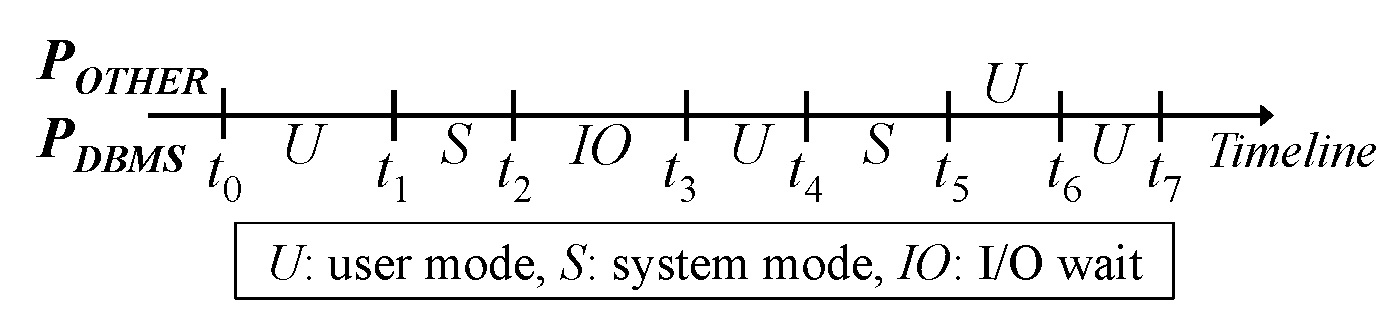
\includegraphics[width=0.48\textwidth]{figures/dbms_time.eps}
\caption{Two interleaved, running processes\label{fig:dbms_time}}
\end{figure}